\usepackage[utf8]{inputenc}
\usepackage{graphicx}
\usepackage{listings}
\usepackage{amsmath}
\usepackage{amssymb}
\usepackage{ae,aecompl}

\usetheme{Goettingen}
\beamertemplatenavigationsymbolsempty

\newcommand{\leftexp}[2]{{\vphantom{#2}}^{#1}{#2}}

\title{3 dimensional D-symbols and the Thurston conjecture}
\author{Boróczki, Lajos}
\date{October 25, 2011}

\begin{document}

\begin{frame}
  \maketitle
\end{frame}

\begin{frame}
  \mode<presentation>{\frametitle{Outline}}
  \tableofcontents
\end{frame}
\newpage

\section{D-symbols}
\begin{frame}
  \frametitle{D-symbol, an algebraic way to describe tilings}
  \begin{itemize}
    \item Based on the baricentric subdivision of a tiling
    \item Structure:
      \begin{itemize}
	\item D-diagram: $dim+1$ colored graph, which represents adjacencies of
	  simplex-orbits
	\item Matrix function on simplex orbits, which represents the number of
	  simpleces (not orbits) around a $dim-2$ dimensional edge
      \end{itemize}
    \item Constraints:
      \begin{itemize}
	\item Compatibility between the diagram and the matrix function
	\item Compatibility with baricentric subdivision
	\item Lower dimensional constraints
      \end{itemize}
    \item Every "nice" tiling has a corresponding D-symbol which is unambigous
      up to permutation \mode<article>{"Nice" tilings are the ones, whose
      baricentric subdivision has finitely many simplex-orbits and does not have
      ideal simplex-vertices except for "real" vertices or "domain-center"
      vertices.  FIXME pontos kifejezesek}
  \end{itemize}
\end{frame}

\subsection{Example}
\begin{frame}
  One of the simplest tilings of space $\mathbb{E}^3$ is with a square prism.
  It's baricentric subdivision and D-diagram: \mode<article>{figure \ref{abra:hasab_bari}.
  As adjacency relations are defined for every simplex orbit, we can skip
  showing the loops which map the orbits mirroring to a plane.}
  \begin{figure}
    \mode<article>{\caption{\label{abra:hasab_bari} Red:1, blue:2, green:3}}
    \center
    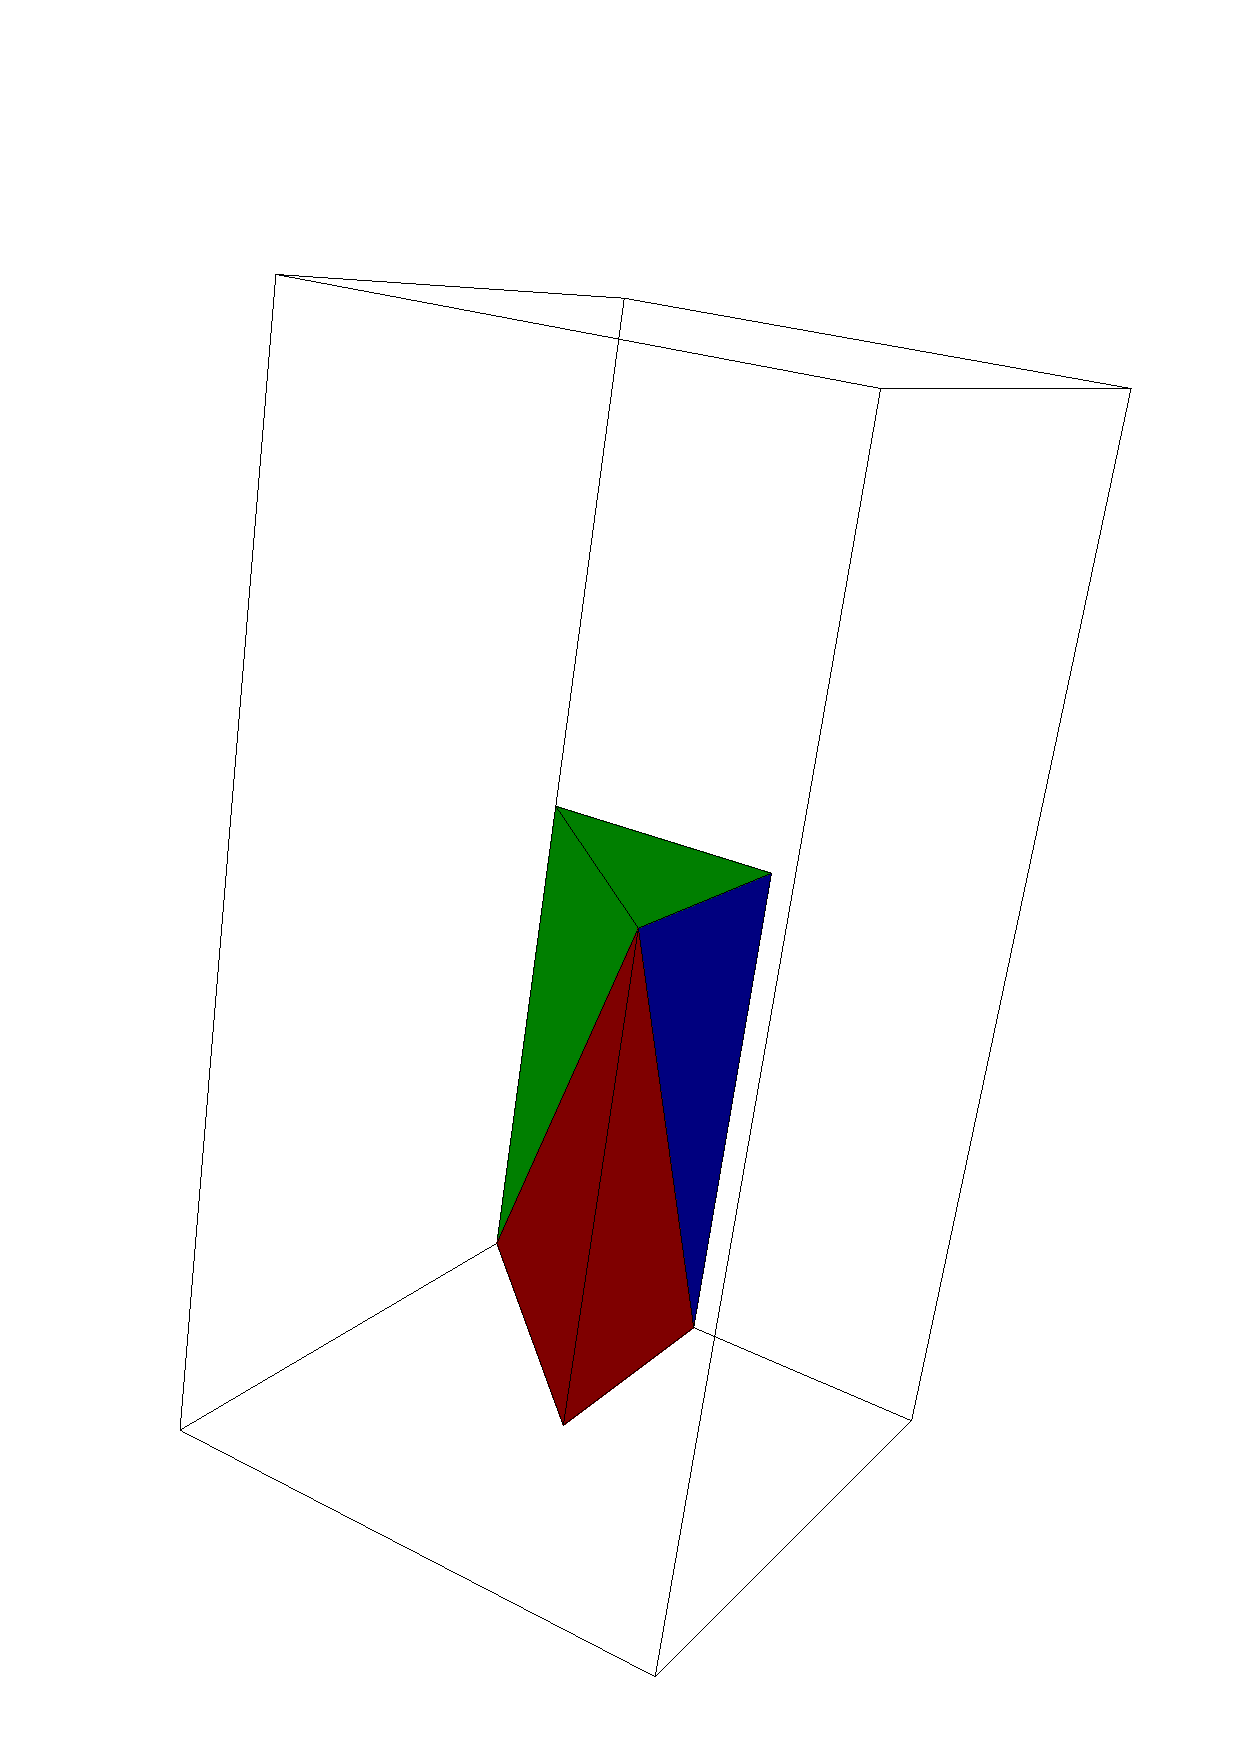
\includegraphics[width=0.4\textwidth]{hasab_bari.pdf}
    \includegraphics[width=0.35\textwidth]{hasab_D-graf.pdf}
  \end{figure}
  Notation:\\<all>
  \setlength{\unitlength}{1cm}
  $\sigma_0$:
  \begin{picture}(1,0.2)
    \multiput(0,0.1)(0.2,0){5}{\circle*{0.001}}
  \end{picture},
  $\sigma_1$:
  \begin{picture}(1,0.2)                                                                                 
    \multiput(0,0.1)(0.25,0){4}{\line(1,0){0.15}}                                                        
  \end{picture},
  $\sigma_2$:
  \begin{picture}(1,0.2)
    \put(0,0.1){\line(1,0){1}}
  \end{picture},
  $\sigma_3$:
  \begin{picture}(1.5,0.2)
    \multiput(0,0.1)(0.5,0){3}{\line(1,0){0.2}}
    \multiput(0.35,0.1)(0.5,0){3}{\circle*{0.001}}
  \end{picture}
\end{frame}

\begin{frame}
  $\mathcal{R}$ and $\mathcal{M}$ matrix-functions (where $\mathcal{D}$ is the set
  of simplex-orbits, $D_i\in\mathcal{D}$):
  \begin{equation*}
    \mathcal{R}(D_1)=
    \left(
    \begin{array}{cccc}
      1 & 1 & 2 & 1\\
      1 & 1 & 3 & 1\\
      2 & 3 & 1 & 2\\
      1 & 1 & 2 & 1
    \end{array}
    \right)
  \end{equation*}
  \begin{equation*}
    \mathcal{R}(D_2)=
    \left(
    \begin{array}{cccc}
      1 & 2 & 2 & 1\\
      2 & 1 & 3 & 2\\
      2 & 3 & 1 & 2\\
      1 & 2 & 2 & 1
    \end{array}
    \right)
  \end{equation*}
  \begin{equation*}
    \mathcal{R}(D_3)=
    \left(
    \begin{array}{cccc}
      1 & 2 & 1 & 1\\
      2 & 1 & 3 & 2\\
      1 & 3 & 1 & 1\\
      1 & 2 & 1 & 1
    \end{array}
    \right)
  \end{equation*}

  \begin{equation*}
    \forall D_i\in\mathcal{D}:\;
    \mathcal{M}(D_i)=
    \left(
    \begin{array}{cccc}
      1 & 4 & 2 & 2\\
      4 & 1 & 3 & 2\\
      2 & 3 & 1 & 4\\
      2 & 2 & 4 & 1
    \end{array}
    \right)
  \end{equation*}
\end{frame}

\section{Constraints for D-symbols}
The following constraints are needed for a D-symbol to have a corresponding
tiling.

\subsection{General constraints}
\begin{frame}
  D-symbol: $(\Sigma_I,\mathcal{D},\mathcal{M})$ triplets. \mode<article>{Where
  $I$ is the index set of the dimension ($|I|=dim+1$), $\Sigma_I$ is the set of
  adjacency operations (interpreted accordingly on the simplex-orbits and the
  simpleces), $\mathcal{D}$ is the set of simplex-orbits and $\mathcal{M}$ is
  the matrix-function on simpleces. These are the Delone-Delaney-Dress symbols,
  briefly D-symbols.}
  \begin{itemize}
    \item Natural constraints for D-diagrams:
      \begin{enumerate}
	\item $\mathcal{D}$ is finite
	\item Adjacency operations on simplex-orbits are involutive 
	  permutations\mode<article>{, this means $\forall i\in I, \sigma_i\in
	  \Sigma_I, \forall D\in \mathcal{D}$:
	  \begin{align*}
	    \sigma_i\sigma_i(D)=D 
	  \end{align*}
	  The degree of the uniformly colored edges in every vertice of the
	  diagram is 1 or 2. It is 2 iff the edge is a loop.}
	\item Using not neighbouring operation-pairs we get back to the starting
	  vertice in at most $2$ steps\mode<article>{. \newline $\forall
	  i,j\in I, \forall D\in \mathcal{D}$:
	  \begin{align*}
	    |i-j|\geq 2 \Rightarrow (\sigma_j\sigma_i)^2(D)=D
	  \end{align*}}
      \end{enumerate}
    \item We can calculate the $\mathcal{R}$ matrix function\mode<article>{,
      which is the same for simplex-orbits as the $\mathcal{M}$ matrix function
      for simpleces: \newline $\forall i,j\in I, \forall D\in \mathcal{D}$:
      \begin{align*}
	r_{ij}(D)=r_{ji}(D)=\mathrm{min}\left\{r\in \mathbb{N}^+|(\sigma_j\sigma_i)^r(D)=D\right\}
      \end{align*}
      Constraints of the D-diagram on $\mathcal{R}$ matrix-function:
      $r_{ii}(D)=1$, and $|i-j|\geq 2 \Rightarrow r_{ij}(D)\leq2$}
    \item Constraints of the $\mathcal{M}$ matrix function:
      \begin{enumerate}
	\item Every element of $\mathcal{R}$ has to divide the appropriate
	  element of $\mathcal{M}$ (parameters)\mode<article>{. Because we have to get to the
	  same simplex walking around a $d-2$ dimensional face (which is an edge
	  in $3$ dimensions,) which means we have to get to the same
	  simplex-orbit too. The quotient of the elements of $\mathcal{M}$ and
	  $\mathcal{R}$ shows the periodicity of the tiling around the $d-2$
	  dimensional face.
	  \newline $\forall i,j\in I, \forall D\in \mathcal{D}$:
	  $r_{ij}(D)|m_{ij}(D)$
	  }
	\item Orbits of adjacency-operation pairs\mode<article>{. An orbit can
	  be defined for every operation-pair and starting simplex-orbit
	  (diagram-vertex). Elements of $\mathcal{M}$ has to be the same inside
	  such an orbit. The reversed orbit has to contain the same number of
	  simpleces, so the matrices of $\mathcal{M}$ has to be symmetric.
	  \begin{align*}
	    &\forall i,j\in I, \forall D\in \mathcal{D} \\
	    &\mathcal{D}'=\left\{(\sigma_j\sigma_i)^k(D)|k\in
	    \mathbb{N}\right\}\cup\left\{\sigma_i(\sigma_j\sigma_i)^k(D)|k\in
	    \mathbb{N}\right\}\\
	    &\forall D_1,D_2 \in \mathcal{D}'\\
	    &m_{ij}(D_1)=m_{ij}(D_2)=m_{ji}(D_1)=m_{ji}(D_2)
	  \end{align*}
	  }
	\item The values of the main diagonal has to be $1$\mode<article>{,
	  because we have adjacency operations.}
	\item The values of the first diagonal above and below the main has to
	  be $\geq2$\mode<article>{. In case of equality we get
	  degenerated tilings, in which for example digons can be facets. (In
	  case of nice tilings in 3 dimensions every vertex joins at least 3
	  edges and 3 facets, every facet has at least 3 edges and every edge
	  joins 3 facets and 3 bodies.)}
	\item Every other value has to be exactly $2$\mode<article>{, so we stay
	  compatible with baricentric subdivision.}
	  $\forall i,j\in I, \forall D\in \mathcal{D}$:
	  \begin{align*}
	    i=j & \Rightarrow m_{ij}(D)=1 \\
	    |i-j| = 1 &\Rightarrow m_{ij}(D)\geq2 \\
	    |i-j|\geq2 &\Rightarrow m_{ij}(D)=2
	  \end{align*}
      \end{enumerate}
  \end{itemize}
\end{frame}

\subsection{2 dimensional subtilings I.}
\begin{frame}
  From now on we only consider 3 dimensional D-symbols. \newline
  D-subsymbol:
  \begin{itemize}
    \item The $i$-th D-subsymbol 
      $(\Sigma_I^i,\mathcal{D}^i,\mathcal{M}^i)$\mode<article>{ can be got by
      eliminating the $i$-th operation from the diagram and the rows and columns
      of the matrix functions.}
    \item We can calculate the combinatorial curvature function of the subsymbol:
      \begin{align*}
	K(\leftexp{c}{\mathcal{D}}^i)=\sum_{D\in
	\leftexp{c}{\mathcal{D}}^i}\left(-1+\sum_{\substack{0\le j<k\le d \\
	j,k\ne i}}\frac{1}{m_{jk}(D)}\right)
	\begin{array}{cccc}
	  > & & S^2 \\
	  = & 0 & \mathbb{E}^2 \\
	  < & & H^2
	\end{array}
      \end{align*}
      \mode<article>{Based on the above formula one can decide, in which $2$
      dimensional constant curvature space realizes the tiling.}
  \end{itemize}
  \mode<presentation>{\begin{minipage}[t]{0.45\textwidth}}
    \begin{itemize}
      \item Good orbifold criteria\mode<article>{: In the above mentioned
	spherical tiling case, we have to exclude bad orbifolds. The following
	options are excluded (given by both Convay's and Macbeath's notations):
	\begin{align*}
	  u=(+,0;[u];\{\}), & & 1<u;\\
	  *u=(+,0;[];\{(u)\}), & & 1<u;\\
	  uv=(+,0;[u,v];\{\}), & & 1<u<v;\\
	  *uv=(+,0;[];\{(u,v)\}), & & 1<u<v.
	\end{align*}}
      \item Visualization:
	\mode<article>{The subsymbol corresponds to the $(3-1)$
	dimensional tiling around the $i$-indexed vertice-class inducated by the
	original D-symbol. So we have to get a spherical tiling around a real
	simplex-vertice (see Fig. \ref{fig:spherical_ex}), or a Euclidean tiling
	around an ideal simplex-vertex in the original tiling. We should not get
	hyperbolic tilings around a simplex-vertex, because this would mean an
	out-of-model vertex.}
    \end{itemize}
  \mode<presentation>{\end{minipage}
  \begin{minipage}[t]{0.5\textwidth}}
    \begin{figure}
      \mode<article>{\caption{\label{fig:spherical_ex}Spherical tiling around
      a simplex-vertex}
      \center
      \includegraphics[width=0.4\textwidth]{d3c3_2_vertice.pdf}}
      \mode<presentation>{\includegraphics[width=0.8\textwidth]{d3c3_2_vertice.pdf}}
    \end{figure}
  \mode<presentation>{\end{minipage}}
\end{frame}

\begin{frame}
  Further constraints in $3$ dimensional D-symbols based on $2$ dimensional
  subsymbols:
  \begin{enumerate}
    \item For $(\Sigma_I^1,\mathcal{D}^1,\mathcal{M}^1)$ and
      $(\Sigma_I^2,\mathcal{D}^2,\mathcal{M}^2)$ the combinatorial curvature
      function has to be positive and the tiling has to be good
      orbifold\mode<article>{. Edge- and face-centered simplex-vertices has to
      be real vertices, so the tiling around them has to be an $S^2$ tiling.}
    \item For $(\Sigma_I^0,\mathcal{D}^0,\mathcal{M}^0)$ and
      $(\Sigma_I^3,\mathcal{D}^3,\mathcal{M}^3)$ the combinatorial curvature 
      function has to be non-negative, and if positive the tiling has to be good
      orbifold\mode<article>{. Vertex- and body-centered simplex-vertices can be
      real or ideal vertices, so the tiling around them can be an $S^2$ or an
      $\mathbb{E}^2$ tiling. (We do not exclude ideal body-centers because of
      the duality.)}
  \end{enumerate}
  These constraints lead to an upper bound of the parameters \mode<article>{as a
  system.}
\end{frame}

\section{2 dimensional subtilings II.}

\begin{frame}
  Splitting probléma és a Thurston-sejtés (támadása)
  Thurston sejtés:
  \begin{itemize}
    \item Minden irányított, primitív, zárt 3-sokaság felvágható (splitting)
      tórusz ($E^2$) felületek mentén úgy, hogy a kapott sokaságok belsejének
      geometriai struktúrája van, melynek véges a térfogata.
    \item A következő 8 féle maximális modell-geometria létezik, amihez van
      kompakt sokaság, ami az adott geometriában modellezhető: $S^3$, $E^3$,
      $H^3$, $S^2\times R$, $H^2\times R$, $\widetilde{SL2R}$, Sol,
      Nil.
  \end{itemize}
  Megjegyzések:
  \begin{itemize}
    \item A nem irányítható eset kezelhető az ,,irányítható dupla fedés''
      módszerrel, ami az M sokasághoz rendelt $M\times Z/2Z$ sokaság
      (értelmes visszahúzó operációval). \mode<article>{Például Möbius szalaghoz
      rendelhetünk egy dupla Möbius szalagot úgy, hogy felvágjuk valahol és
      betoldunk mégegy Möbius szalagot. Ezzel egy gyűrű alakot kapunk.}
    \item A 2 dimenziós analógia: minden határ nélküli felületnek (2-sokaságnak)
      geometriai struktúrája van, konstans görbületű metrikával.
  \end{itemize}
\end{frame}

\begin{frame}
  Splitting keresése D-szimbólumban
  \begin{itemize}
    \item $S^2$ jellegű splitting: Ponttá zsugorítható részlet a kövezésben,
      ezáltal \mode<article>{kevesebb szimplex-csúcsból, így} kevesebb
      szimplex-pályából álló kövezéssel ekvivalenset kapunk. (Rossz orbifold
      probléma itt is felléphet.)
      FIXME Rajz
    \item $E^2$ splitting: A Thurston sejtés-beli splittingnek megfelelő dolog.
      Végtelen távoli pontba tolható.
      FIXME Rajz
  \end{itemize}
\end{frame}

\begin{frame}
  További feltételek a Thurston sejtés-beli minimális 3-sokaságokra
  \begin{itemize}
    \item Az ábrákon látszik, hogy a megfelelő 2 sokaságokra a kombinatorikus
      görbület függvényt felírva alsó korlátot is kapunk a paramétereinkre.
      FIXME Fontos kérdés, hogy ez elég-e.
    \item A D-diagram alapján felírhatóak a szimplex csúcsok (rész D-diagram) és
      a szimplex csúcsok közti élek is. Ezeket gráfnak tekintve az összes
      lehetséges 2 (legalább 2 elemű) partícióra bontást meg kell vizsgálni.
    \item Az így kapott "splitting-jelölt" helyet meg kell vizsgálni, hogy
      megkapjuk az összes alsó korlátot a paraméterekre.
    \item A kapott D-szimbólumok minimálisak abban az értelemben, hogy nincs
      bennük se $E^2$ se $S^2$ splitting. (Ha találunk köztük olyat, ami nem
      realizálható a 8-féle geometriában, akkor a Thurston-sejtést sikeresen
      támadtuk.)
  \end{itemize}
\end{frame}


\section{Enumerating D-symbols}
\begin{frame}
  D-szimbólumok felsorolása:
  \begin{itemize}
    \item Nagyravágyó terv\mode<article>{: Az összes $n$-dimenziós geometriában
      az összes lehetséges véges alaptartományú kövezés felsorolásához
      szeretnénk a D-szimbólumokat felhasználni.}
    \item Alapvetően nem tűnik lehetetlennek\mode<article>{, mivel a
      D-szimbólumokat minden olyan kövezésre értelmezhetjük, ahol tudunk
      baricentrikus felbontást végezni.}
    \item Nagyon sok lehetőség van\mode<article>{: a dimenzió és a D-diagram
      elemszámának méretében is exponenciális}
    \item Rendezés a D-diagramokon, algoritmus a felsorolásukra
    \item Rendezés a mátrix-függvényeken, $3$-dimenziós esetben algoritmus a
      lehetséges mátrix-függvények felsorolására \mode<article>{ az előző
      fejezetben felsorolt feltételeknek megfelelően. A két kulcs a paraméteres
      megadás és a rész D-szimbólum által indukált felső korlát (de a végtelen
      láncokat kezelni kell.)}
    \item A 12 elemszámú D-szimbólumokat tudjuk jelenleg felsorolni.
  \end{itemize}
\end{frame}

\subsection{Enumerating edge-transitive D-symbols}
\begin{frame}
  Éltranzitív kövezések kezelése D-szimbólummal
  \begin{itemize}
    \item Egyszerű új feltétel: a diagramban nem lehet 1-es színű (szaggatott)
      él
    \item A lehetséges diagramok végigpróbálgatása egyszerűbbé válik
    \item 18-as elemszámig jutottunk, és ismert, hogy legfeljebb 24 elemszámú
      ilyen diagramok lehetségesek.
  \end{itemize}
\end{frame}

\end{document}
